\subsection{Resultados}
Os cenários para teste foram: seleção completa da tabela de usuários (\textit{SELECT *}), seleção do primeiro usuário (\textit{SELECT FIRST}), seleção do último usuário (\textit{SELECT LAST}), criação e deleção de um usuário (\textit{CREATE AND DELETE}), seleção condicional de um usuário (\textit{SELECT WHERE}) e seleção ordenada de usuários (\textit{SELECT ORDER}). Os resultados desses testes, abarcando uma variedade de contextos pertinentes à utilização de ORMs, são apresentados a seguir.

\begin{figure}[H]
    \centering
    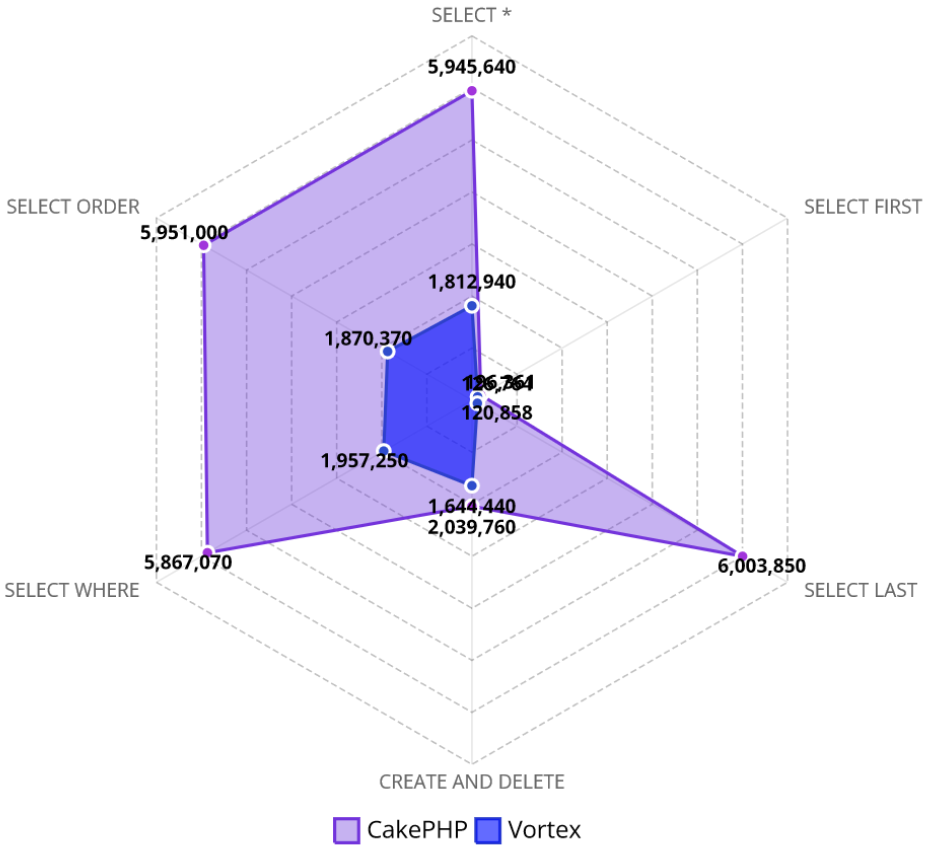
\includegraphics[width=0.7\linewidth]{figures/vortex_vs_cakephp.png}
    \caption{Gráfico comparativo performance ORM CakePHP e Vortex}
    \label{fig:vortex_vs_cakephp}
\end{figure}

\begin{table}[H] \footnotesize
\fontsize{9pt}{9pt}\selectfont
\centering
\vspace{1cm}
\begin{tabular}{|c|c|c|c|}
\hline  
& Vortex & CakePHP & CakePHP / Vortex\\
\hline 
SELECT * & 1812940 ns & 5945640 ns & $\approx$ 3,279x \\
SELECT FIRST & 126764 ns  & 196361 ns & $\approx$ 1,549x \\
SELECT LAST & 120858 ns  & 6003850 ns & $\approx$ 49,676x \\
CREATE AND DELETE & 1644440 ns & 2039760 ns & $\approx$ 1,240x \\
SELECT WHERE & 1957250 ns & 5867070 ns & $\approx$ 2,997x \\
SELECT ORDER & 1870370 ns & 5951000 ns & $\approx$ 3,181x \\
\hline
\end{tabular}
\caption{Proporcionalidade na performance entre \textit{frameworks}: análise do número de vezes em que o Vortex supera o CakePHP em testes controlados}
\label{vortex_vs_cakephp}
\end{table}

\begin{figure}[H]
    \centering
    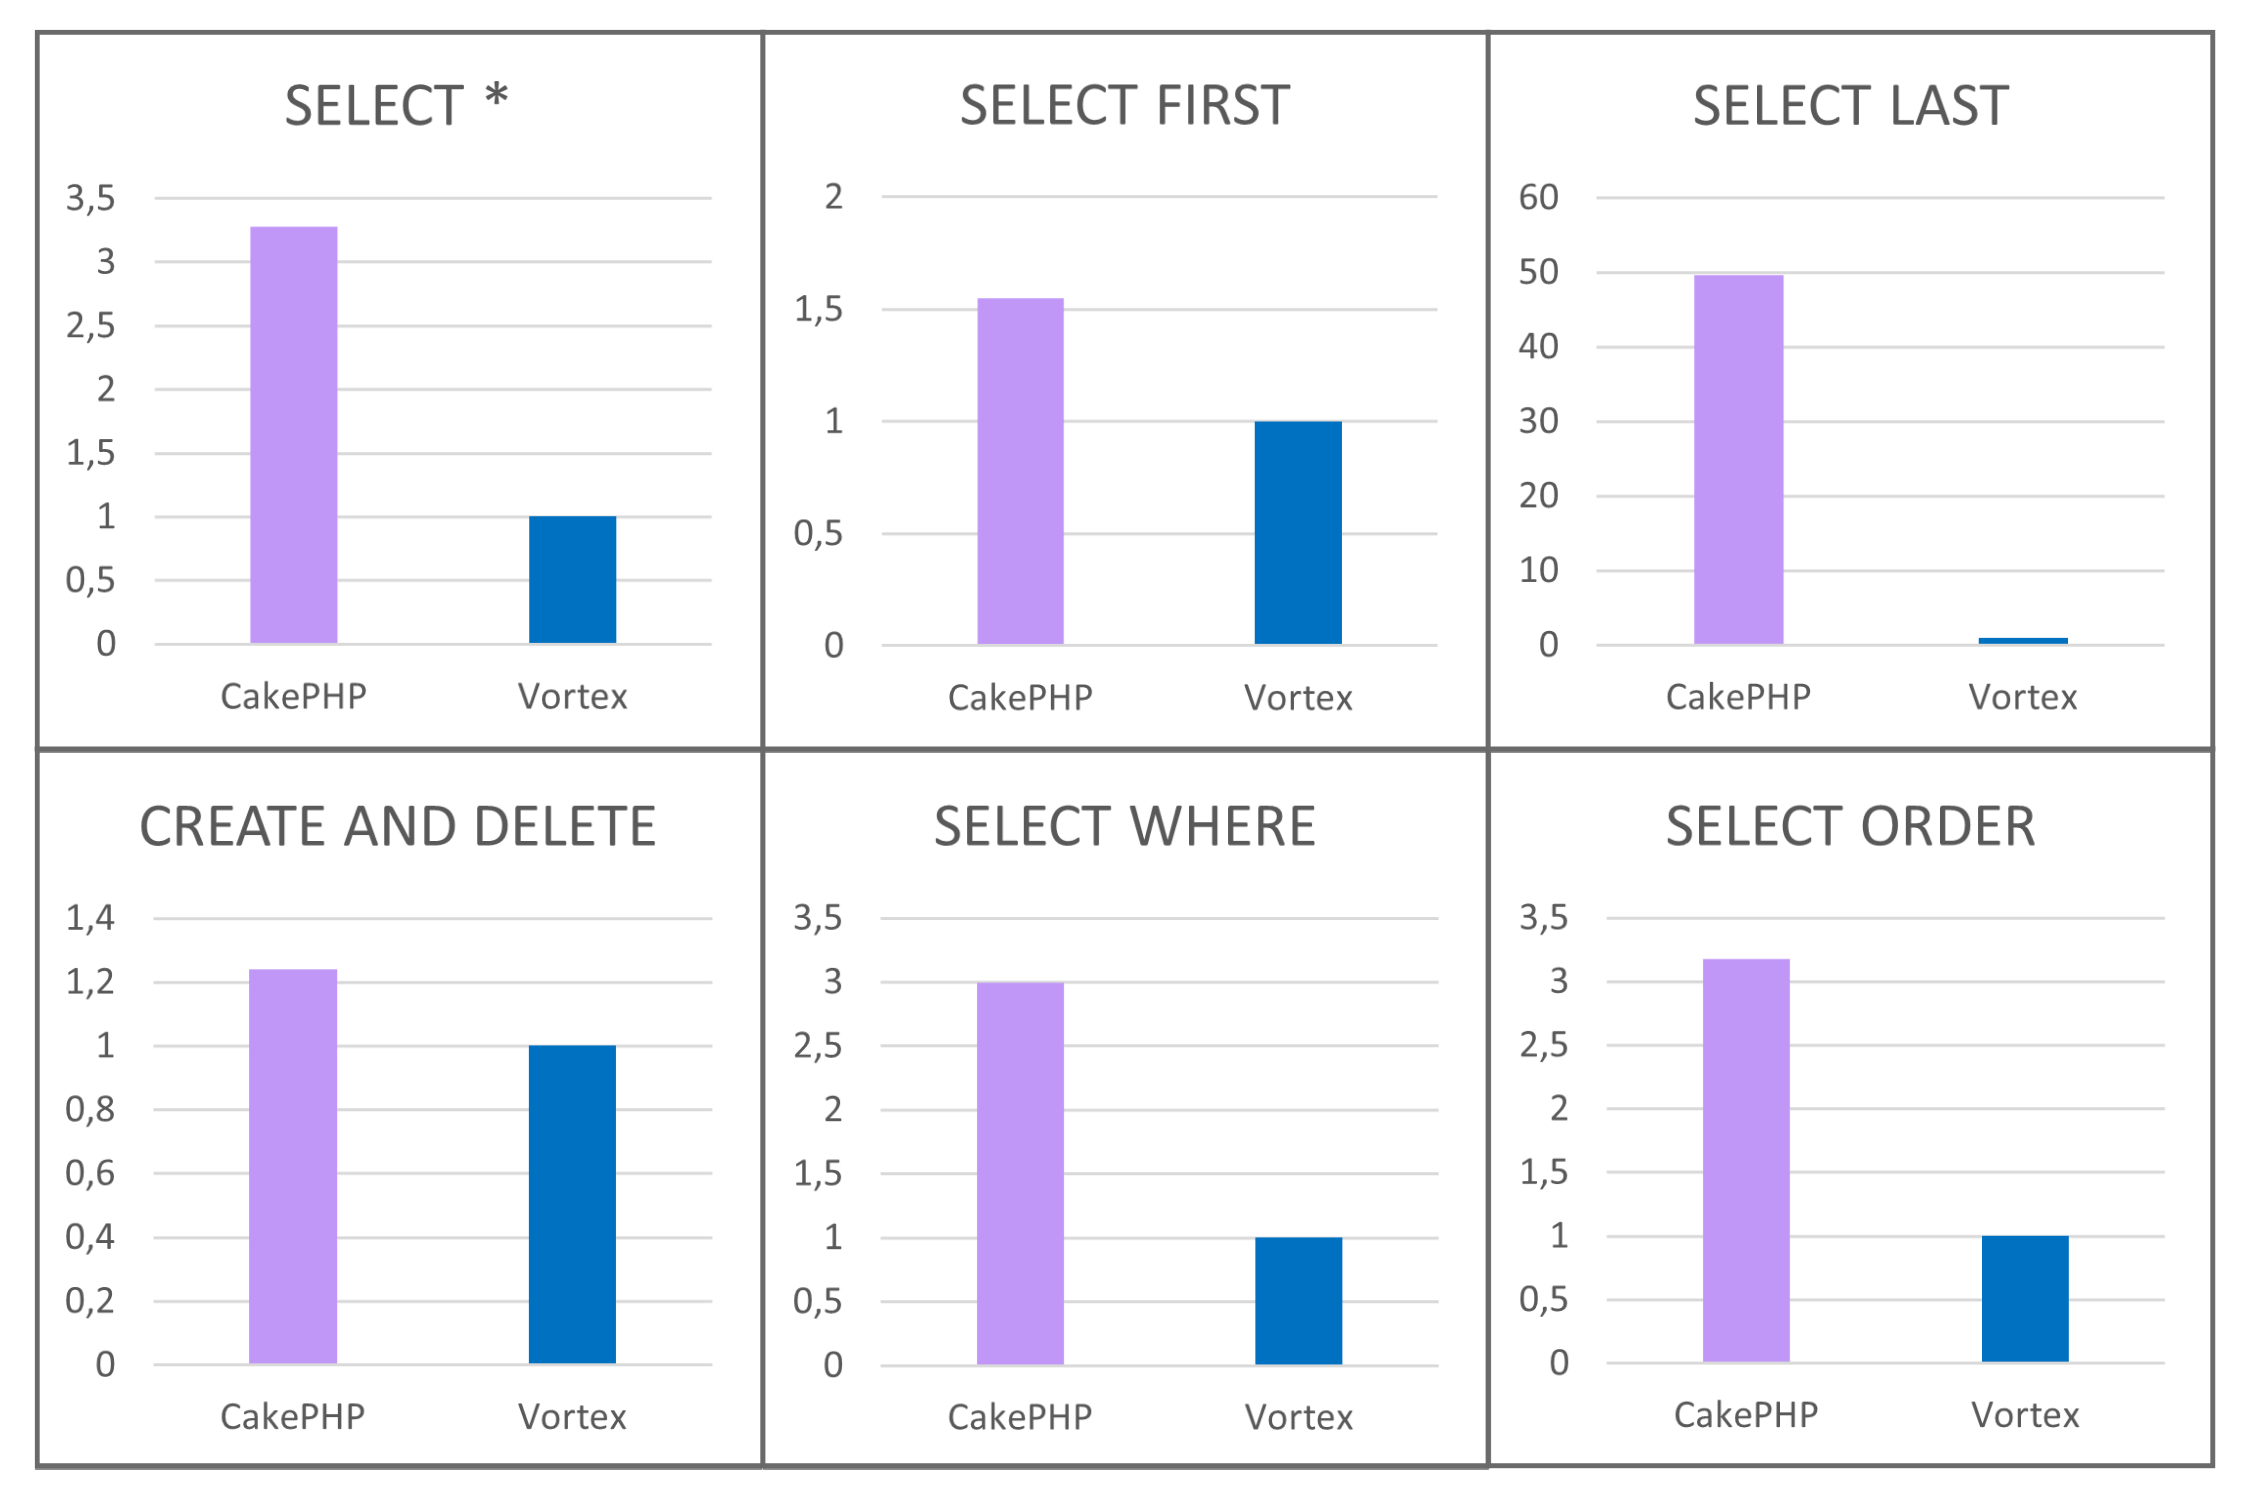
\includegraphics[width=0.9\linewidth]{figures/vortex_vs_cakephp_barcode.png}
    \caption{Gráfico comparativo performance ORM CakePHP e Vortex}
    \label{fig:vortex_vs_cakephp_barcode}
\end{figure}

A análise dos dados gerados mediante a comparação entre o CakePHP e o Vortex, conforme ilustrado nas Figuras \ref{fig:vortex_vs_cakephp},  \ref{fig:vortex_vs_cakephp_barcode}, bem como sumarizado na Tabela \ref{vortex_vs_cakephp}, revela as seguintes constatações:

\begin{enumerate}
    \item Na execução da consulta completa utilizando a cláusula \textit{SELECT *}, observou-se que o CakePHP manifestou um desempenho aproximadamente $\approx$ 3,279 vezes mais custoso. 
    \item Ao direcionar a consulta para recuperar o primeiro registro  \textit{SELECT FIRST}, constatou-se que o CakePHP apresentou um custo aproximado de $\approx$ 1,549 vezes superior em relação ao Vortex. 
    \item A realização da consulta para obter o último registro \textit{SELECT LAST} revelou um desproporcional incremento no tempo de execução pelo CakePHP, alcançando um custo aproximadamente $\approx$ 49,676 vezes maior em comparação ao Vortex.
    \item No contexto da criação e deleção de um usuário \textit{CREATE AND DELETE}, constatou-se que o CakePHP implicou em um custo aproximado de $\approx$ 1,240 vezes superior.
    \item Nas consultas condicionais \textit{SELECT WHERE}, o CakePHP apresentou um custo aproximadamente $\approx$ 2,997 vezes mais elevado.
    \item Em consultas ordenadas \textit{SELECT ORDER}, verificou-se que o CakePHP registrou um custo aproximadamente $\approx$ 3,181 vezes superior em comparação ao Vortex.
\end{enumerate}

\begin{figure}[H]
    \centering
    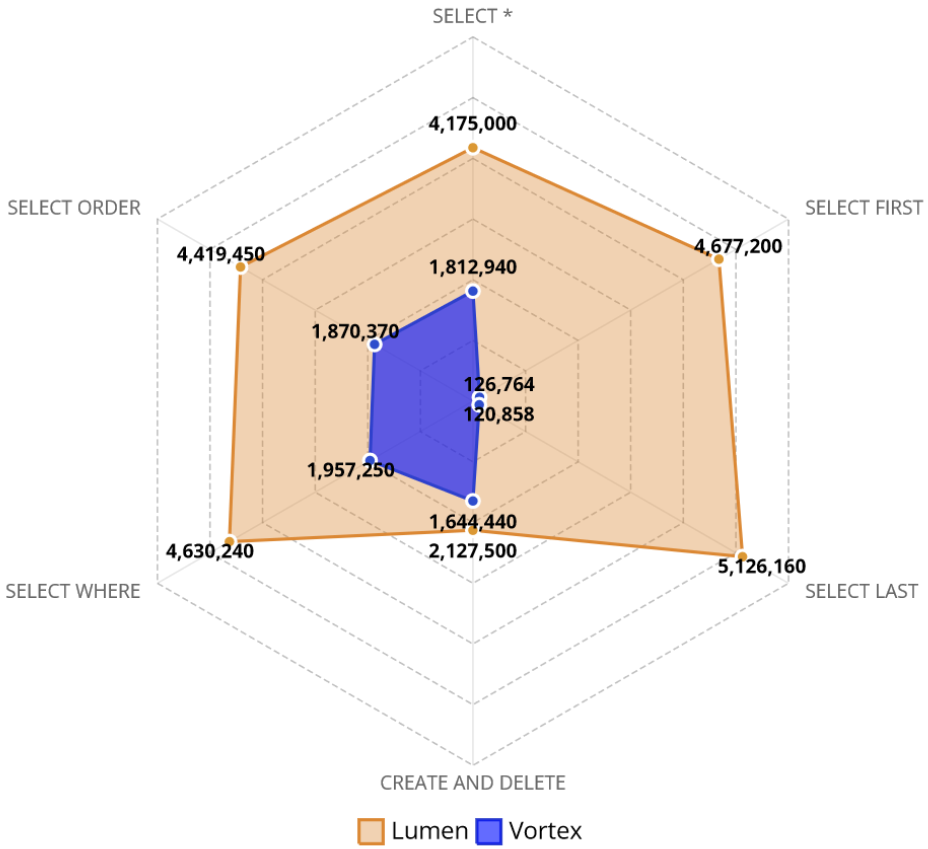
\includegraphics[width=0.7\linewidth]{figures/vortex_vs_lumen.png}
    \caption{Gráfico comparativo performance ORM Lumen e Vortex}
    \label{fig:vortex_vs_lumen}
\end{figure}

\begin{table}[H] \footnotesize
\fontsize{9pt}{9pt}\selectfont
\centering
\vspace{1cm}
\begin{tabular}{|c|c|c|c|}
\hline  
& Vortex & Lumen & Lumen / Vortex\\
\hline 
SELECT * & 1812940 ns & 4175000 ns & $\approx$ 2,302x \\
SELECT FIRST & 126764 ns  & 4677200 ns & $\approx$ 36,896x \\
SELECT LAST & 120858 ns  & 5126160 ns & $\approx$ 42,414x \\
CREATE AND DELETE & 1644440 ns & 2127500 ns & $\approx$ 1,293x \\
SELECT WHERE & 1957250 ns & 4630240 ns & $\approx$ 2,365x \\
SELECT ORDER & 1870370 ns & 4419450 ns & $\approx$ 2,362x \\
\hline
\end{tabular}
\caption{Proporcionalidade na performance entre \textit{frameworks}: análise do número de vezes em que o Vortex supera o Lumen em testes controlados}
\label{vortex_vs_lumen}
\end{table}

\begin{figure}[H]
    \centering
    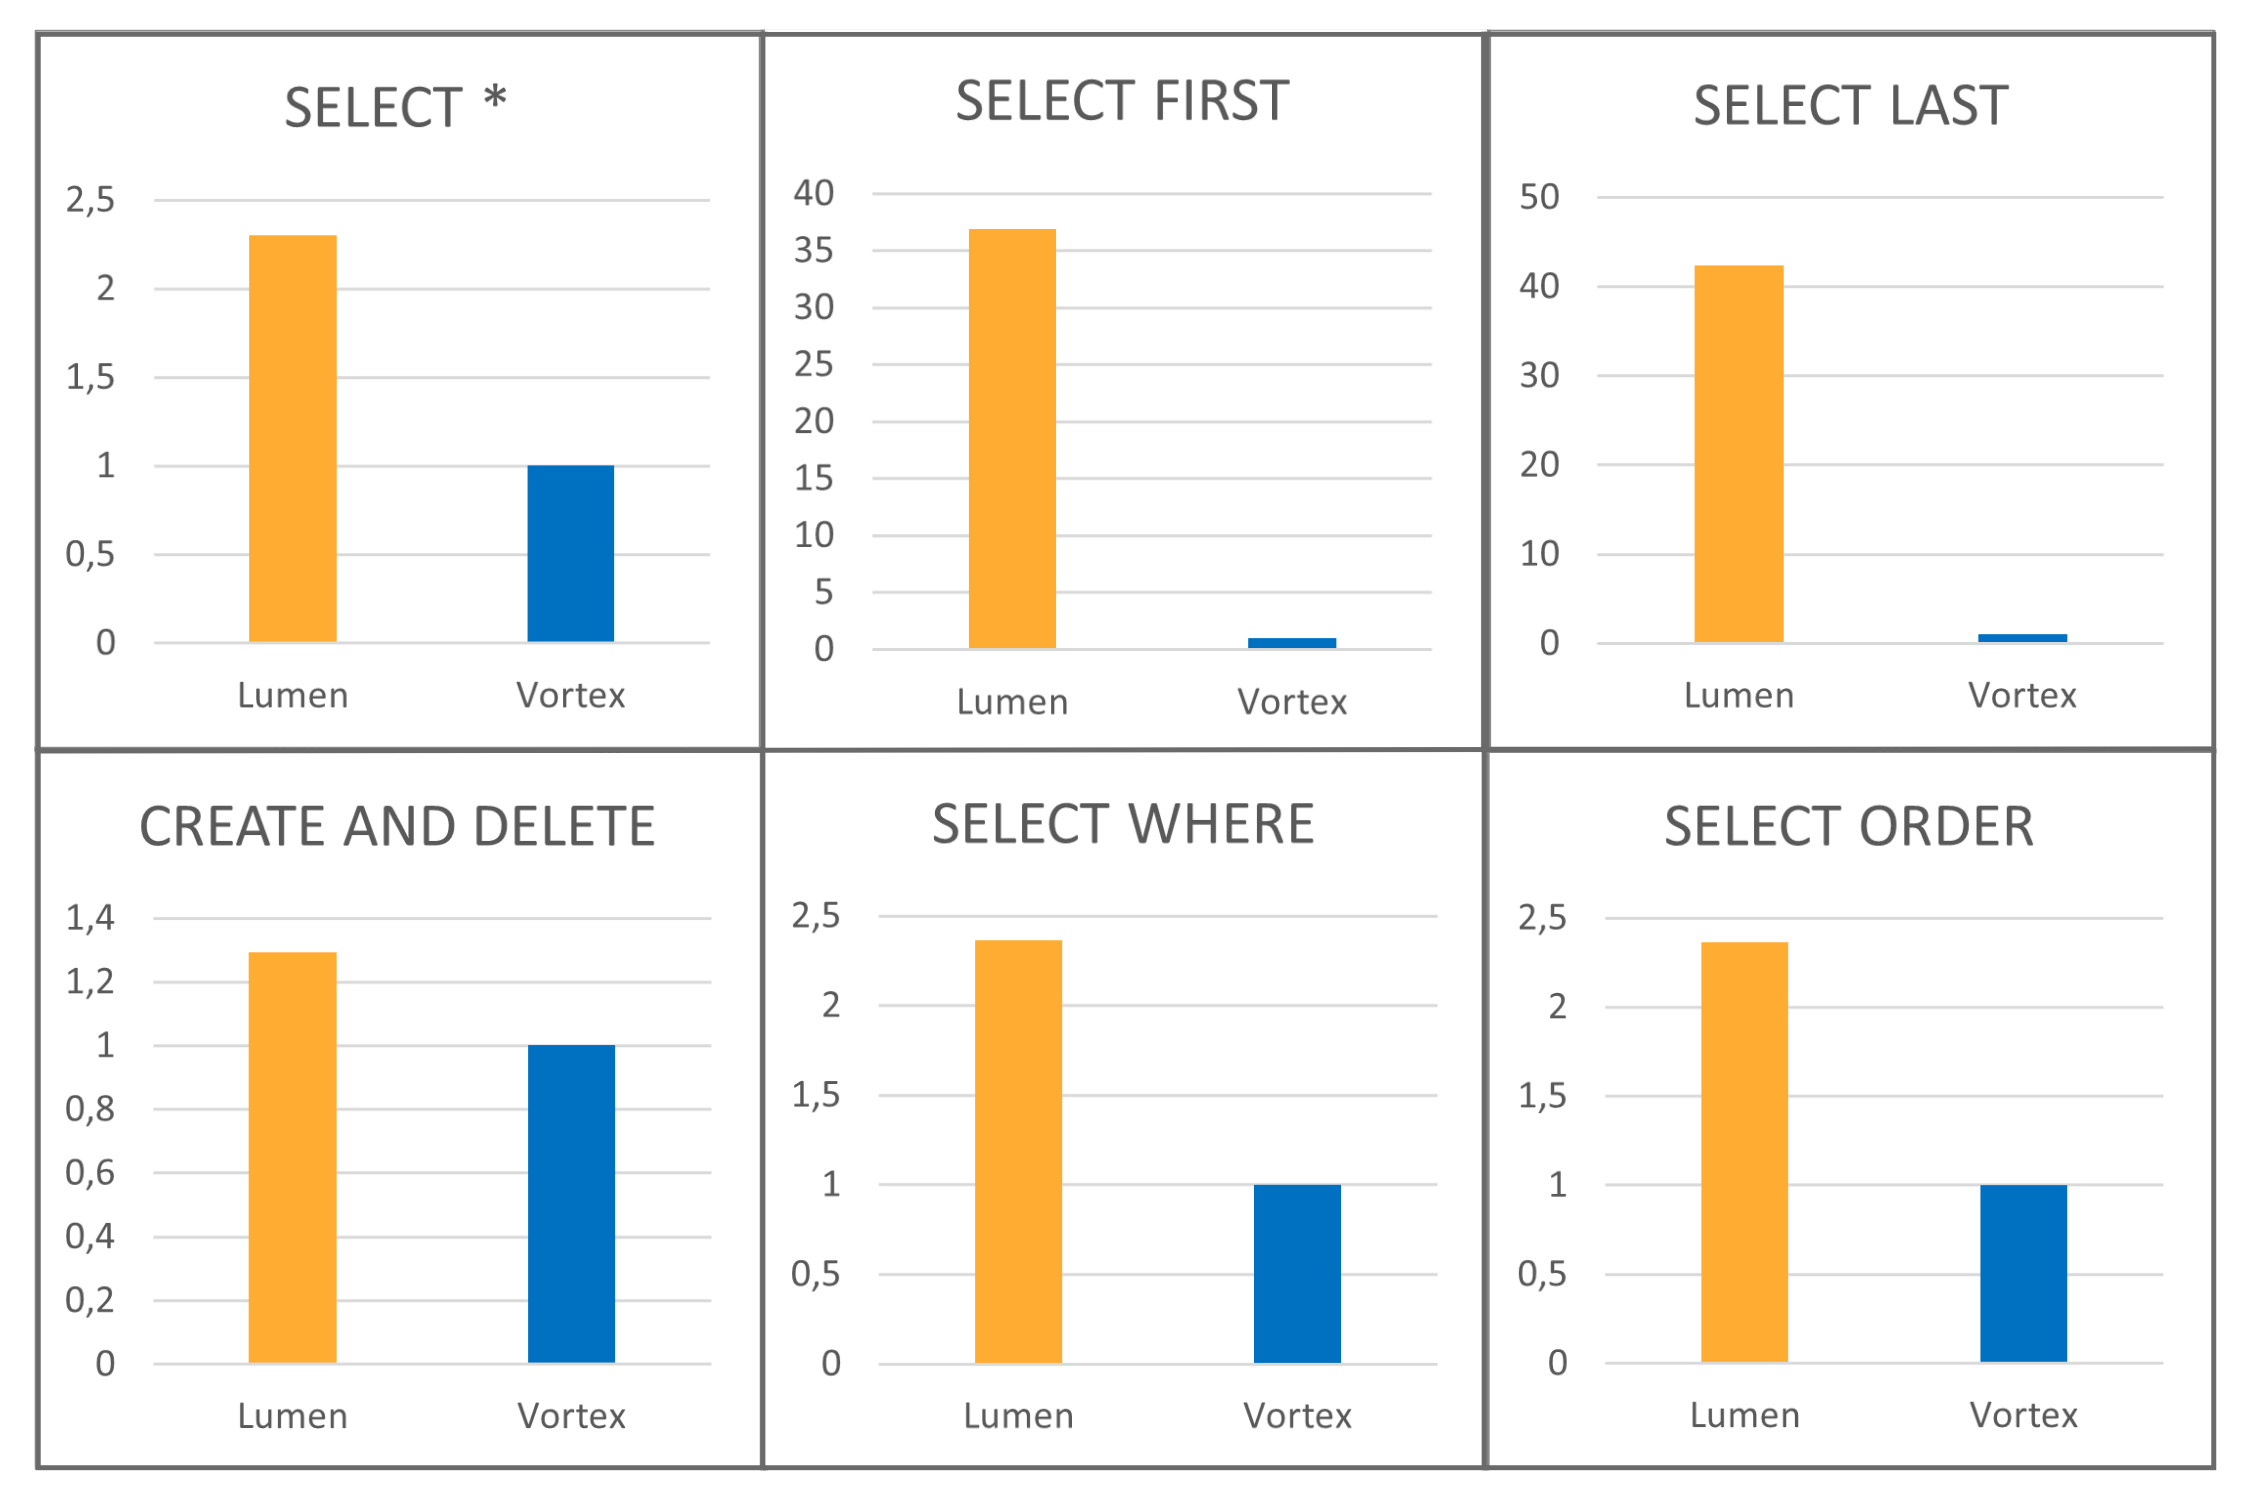
\includegraphics[width=0.9\linewidth]{figures/vortex_vs_lumen_barcode.png}
    \caption{Gráfico comparativo performance ORM Lumen e Vortex}
    \label{fig:vortex_vs_lume_barcode}
\end{figure}

A análise dos dados obtidos por meio da comparação entre o Lumen e o Vortex, conforme evidenciado nas Figuras \ref{fig:vortex_vs_lumen} e \ref{fig:vortex_vs_lume_barcode}, e devidamente sumarizado na Tabela \ref{vortex_vs_lumen}, proporciona revelações significativas:

\begin{enumerate}
    \item No contexto da execução da consulta completa utilizando a cláusula \textit{SELECT *}, observou-se que o Lumen demonstrou um desempenho aproximadamente $\approx$ 2,302 vezes mais dispendioso.
    \item Ao direcionar a consulta para recuperar o primeiro registro (\textit{SELECT FIRST}), verificou-se que o Lumen implicou em um custo aproximado de $\approx$ 36,896 vezes superior em relação ao Vortex.
    \item A condução da consulta para obtenção do último registro (\textit{SELECT LAST}) revelou um notável incremento no tempo de execução pelo Lumen, alcançando um custo aproximadamente $\approx$ 42,414 vezes maior em comparação ao Vortex.
    \item No âmbito da criação e exclusão de um usuário (\textit{CREATE AND DELETE}), constatou-se que o Lumen acarretou um custo aproximado de $\approx$ 1,293 vezes superior.
    \item Nas consultas condicionais (\textit{SELECT WHERE}), o Lumen demonstrou um custo aproximadamente $\approx$ 2,365 vezes mais elevado.
    \item Em consultas ordenadas (\textit{SELECT ORDER}), observou-se que o Lumen registrou um custo aproximadamente $\approx$ 2,362 vezes superior em comparação ao Vortex.
\end{enumerate}

\begin{figure}[H]
    \centering
    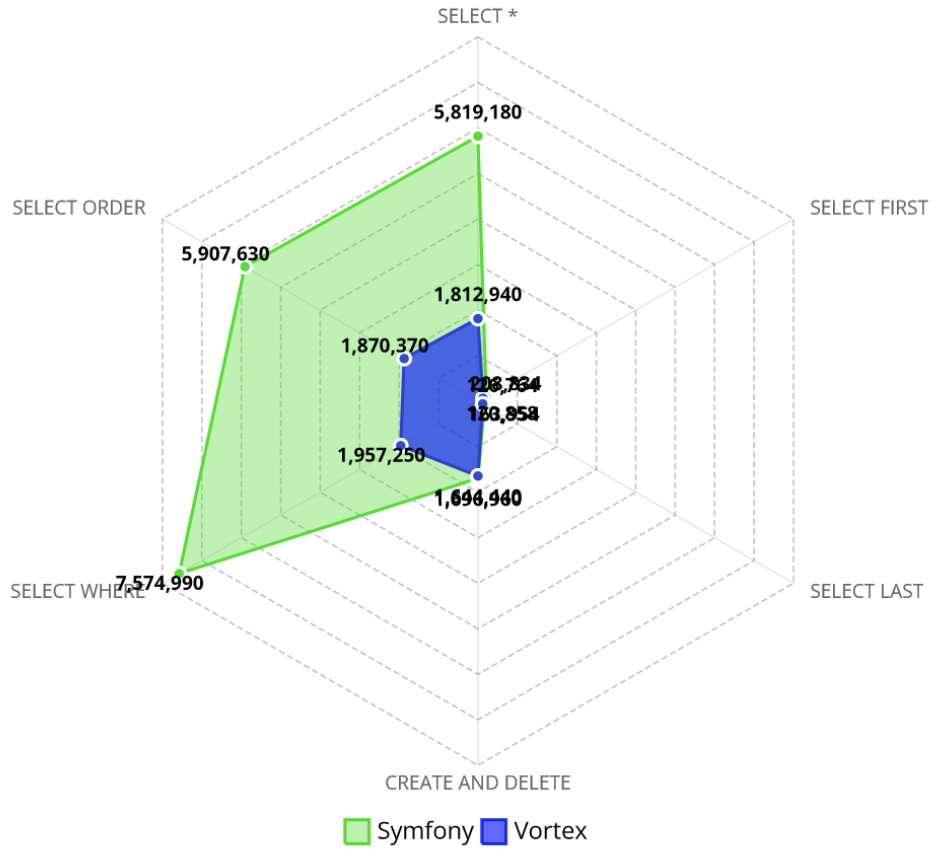
\includegraphics[width=0.7\linewidth]{figures/vortex_vs_symfony.png}
    \caption{Gráfico comparativo performance ORM Symfony e Vortex}
    \label{fig:vortex_vs_symfony}
\end{figure}

\begin{table}[H] \footnotesize
\fontsize{9pt}{9pt}\selectfont
\centering
\vspace{1cm}
\begin{tabular}{|c|c|c|c|}
\hline  
& Vortex & Symfony & Symfony / Vortex\\
\hline 
SELECT * & 1812940 ns & 5819180 ns & $\approx$ 3,209x \\
SELECT FIRST & 126764 ns  & 208834 ns & $\approx$ 1,647x \\
SELECT LAST & 120858 ns  & 163954 ns & $\approx$ 1,356x \\
CREATE AND DELETE & 1644440 ns & 1696960 ns & $\approx$ 1,031x \\
SELECT WHERE & 1957250 ns & 7574990 ns & $\approx$ 3,870x \\
SELECT ORDER & 1870370 ns & 5907630 ns & $\approx$ 3,158x \\
\hline
\end{tabular}
\caption{Proporcionalidade na performance entre \textit{frameworks}: análise do número de vezes em que o Vortex supera o Symfony em testes controlados}
\label{vortex_vs_symfony}
\end{table}

\begin{figure}[H]
    \centering
    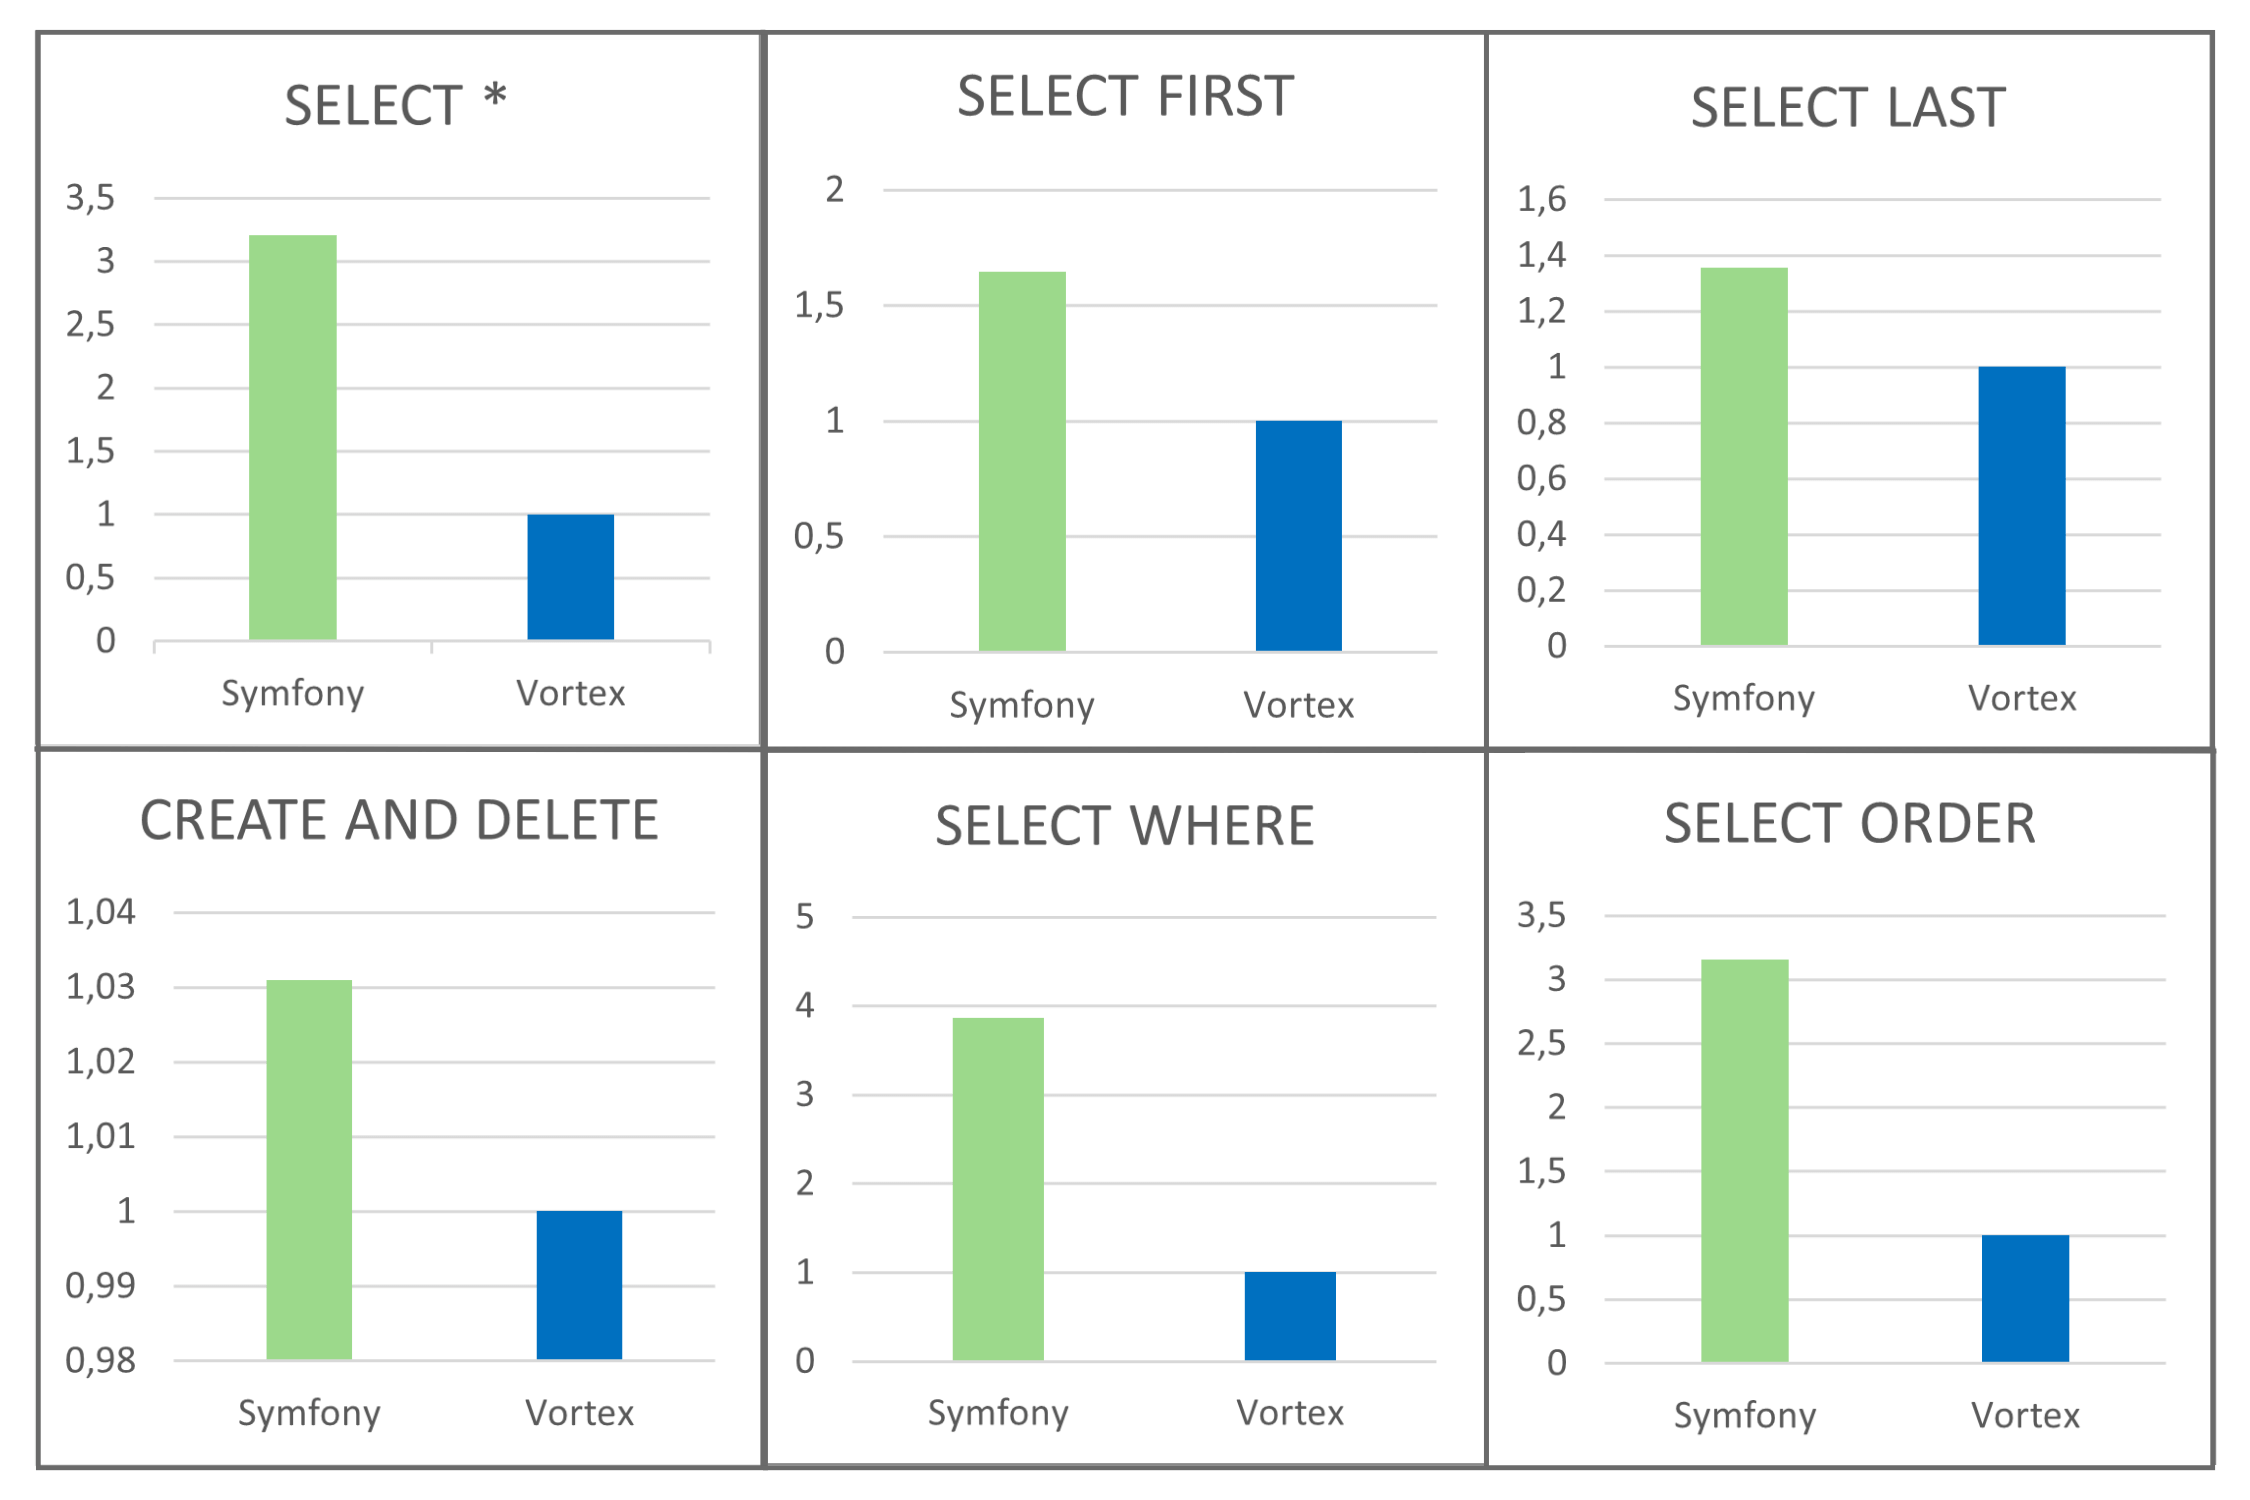
\includegraphics[width=0.9\linewidth]{figures/vortex_vs_symfony_barcode.png}
    \caption{Gráfico comparativo performance ORM Symfony e Vortex}
    \label{fig:vortex_vs_symfony_barcode}
\end{figure}

A análise dos dados decorrentes da comparação entre o Symfony e o Vortex, conforme ilustrado nas Figuras \ref{fig:vortex_vs_symfony} e \ref{fig:vortex_vs_symfony_barcode}, e devidamente resumido na Tabela \ref{vortex_vs_symfony}, proporciona importantes conclusões:

\begin{enumerate}
    \item No contexto da realização da consulta completa utilizando a cláusula \textit{SELECT *}, constatou-se que o \textit{framework} Symfony exibiu um desempenho aproximadamente $\approx$ 3,209 vezes mais oneroso.
    \item Ao focalizar a consulta para recuperar o primeiro registro (\textit{SELECT FIRST}), verificou-se que o Symfony implicou em um custo aproximado de $\approx$ 1,647 vezes superior em relação ao Vortex.
    \item A condução da consulta para obtenção do último registro (\textit{SELECT LAST}) revelou um notável incremento no tempo de execução pelo Symfony, alcançando um custo aproximadamente $\approx$ 1,356 vezes maior em comparação ao Vortex.
    \item No escopo da criação e exclusão de um usuário (\textit{CREATE AND DELETE}), constatou-se que o Symfony acarretou um custo aproximado de $\approx$ 1,031 vezes superior.
    \item Nas consultas condicionais (\textit{SELECT WHERE}), o Symfony manifestou um custo aproximadamente $\approx$ 3,870 vezes mais elevado.
    \item Em consultas ordenadas (\textit{SELECT ORDER}), observou-se que o Symfony registrou um custo aproximadamente $\approx$ 3,158 vezes superior em comparação ao Vortex.
\end{enumerate}


\begin{figure}[H]
    \centering
    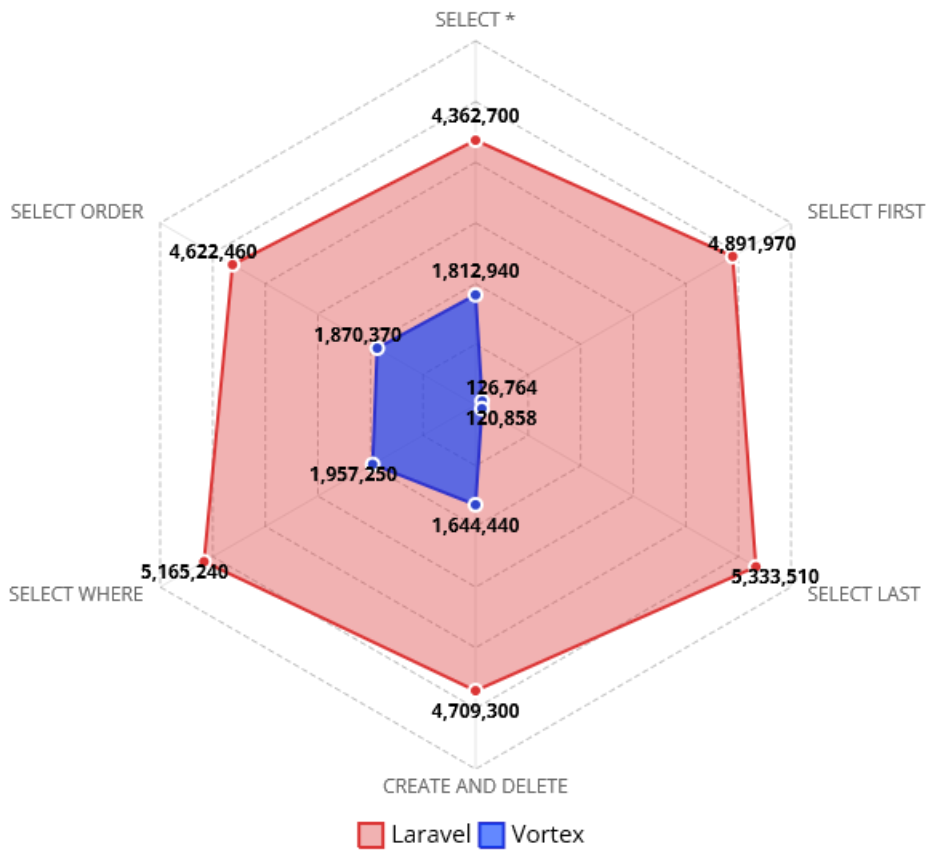
\includegraphics[width=0.7\linewidth]{figures/vortex_vs_laravel.png}
    \caption{Gráfico comparativo performance ORM Laravel e Vortex}
    \label{fig:vortex_vs_laravel}
\end{figure}

\begin{table}[H] \footnotesize
\fontsize{9pt}{9pt}\selectfont
\centering
\vspace{1cm}
\begin{tabular}{|c|c|c|c|}
\hline  
& Vortex & Laravel & Laravel / Vortex\\
\hline 
SELECT * & 1812940 ns & 4362700 ns & $\approx$ 2,406x \\
SELECT FIRST & 126764 ns  & 4891970 ns & $\approx$ 38,591x \\
SELECT LAST & 120858 ns  & 5333510 ns & $\approx$ 44,130x \\
CREATE AND DELETE & 1644440 ns & 4709300 ns & $\approx$ 2,863x \\
SELECT WHERE & 1957250 ns & 5165240 ns & $\approx$ 2,639x \\
SELECT ORDER & 1870370 ns & 4622460 ns & $\approx$ 2,471x \\
\hline
\end{tabular}
\caption{Proporcionalidade na performance entre \textit{frameworks}: análise do número de vezes em que o Vortex supera o Laravel em testes controlados}
\label{vortex_vs_laravel}
\end{table}

\begin{figure}[H]
    \centering
    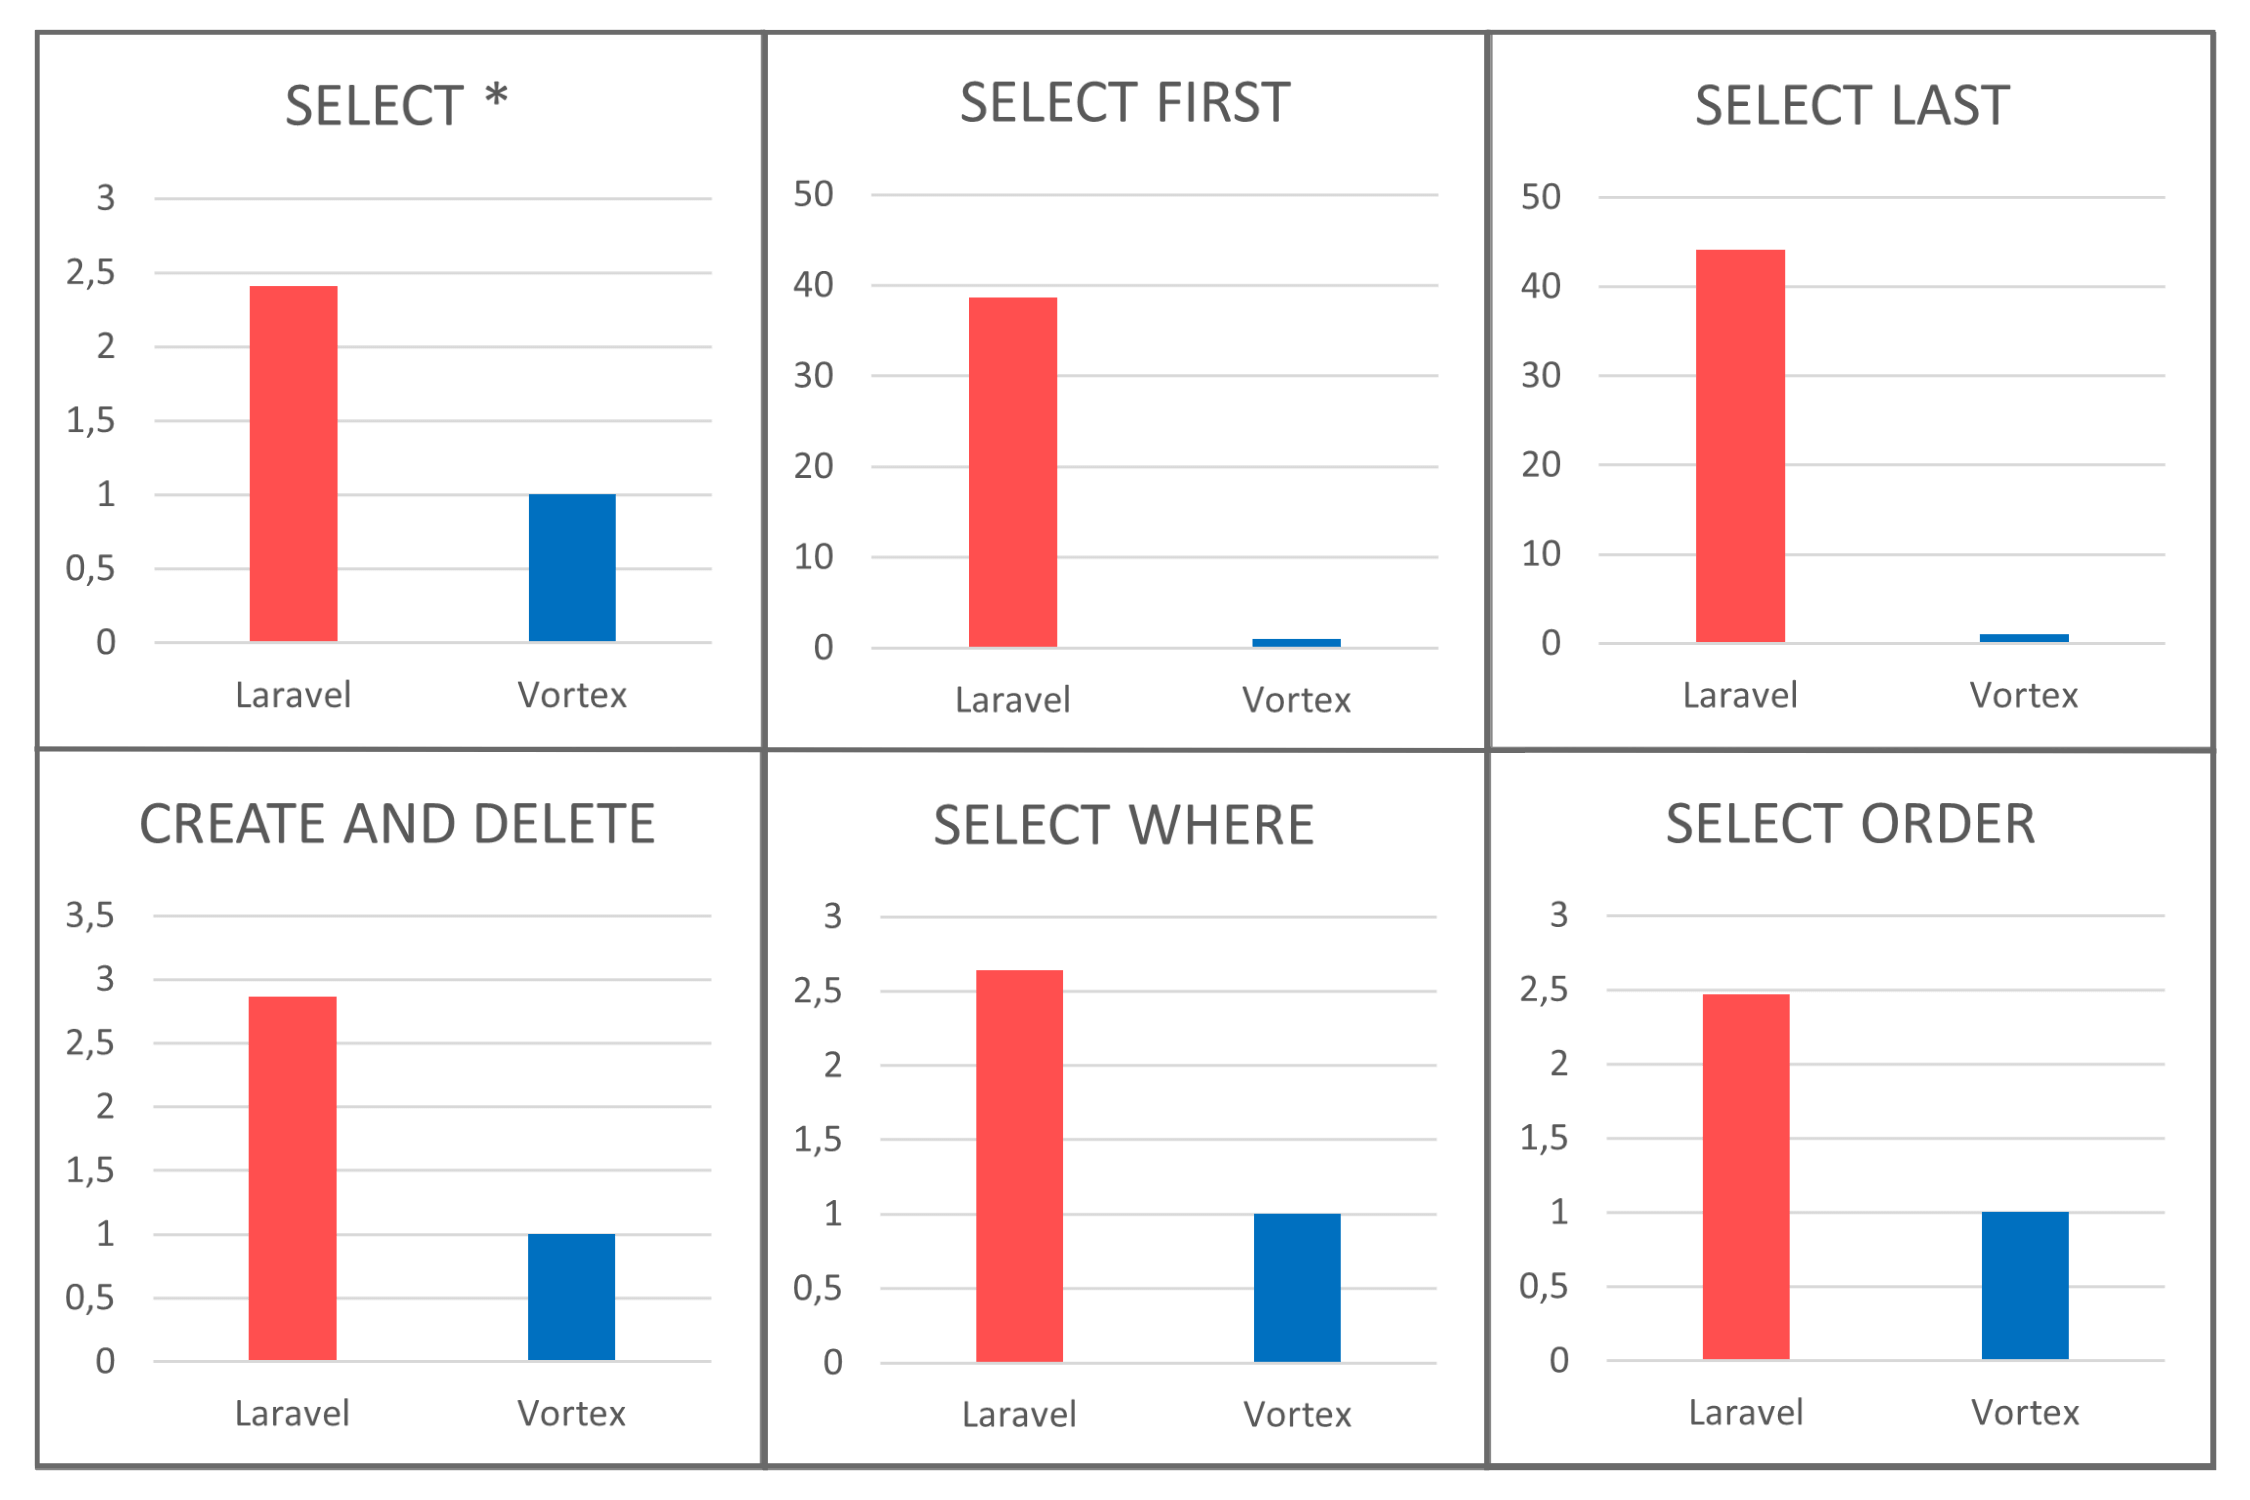
\includegraphics[width=0.9\linewidth]{figures/vortex_vs_laravel_barcode.png}
    \caption{Gráfico comparativo performance ORM Laravel e Vortex}
    \label{fig:vortex_vs_laravel_barcode}
\end{figure}

A avaliação dos dados resultantes da comparação entre o Laravel e o Vortex, conforme representado nas Figuras \ref{fig:vortex_vs_laravel} e \ref{fig:vortex_vs_laravel_barcode}, e devidamente resumida na Tabela \ref{vortex_vs_laravel}, conduz as seguintes conclusões:

\begin{enumerate}
    \item Na execução da pesquisa completa usando a cláusula \textit{SELECT *}, foi observado que o \textit{framework} Laravel demonstrou um desempenho aproximadamente $\approx$ 2,406 vezes mais dispendioso.
    \item Ao direcionar a consulta para recuperar o primeiro registro (\textit{SELECT FIRST}), verificou-se que o Laravel resultou em um custo aproximado de $\approx$ 38,591 vezes superior em relação ao Vortex.
    \item A realização da consulta para obtenção do último registro (\textit{SELECT LAST}) evidenciou um significativo aumento no tempo de execução pelo Laravel, resultando em um custo aproximadamente $\approx$ 44,130 vezes maior em comparação ao Vortex.
    \item No âmbito da criação e exclusão de um usuário (\textit{CREATE AND DELETE}), constatou-se que o Laravel gerou um custo aproximado de $\approx$ 2,863 vezes superior.
    \item Nas consultas condicionais (\textit{SELECT WHERE}), o Laravel revelou um custo aproximadamente $\approx$ 2,639 vezes mais elevado.
    \item Em consultas ordenadas (\textit{SELECT ORDER}), foi observado que o Laravel registrou um custo aproximadamente $\approx$ 2,471 vezes superior em comparação ao Vortex.
\end{enumerate}

De maneira isolada, procedemos à análise das consultas envolvendo relacionamentos, representadas através do uso da cláusula \textit{SELECT WITH}. No âmbito deste estudo, tais consultas se referem à obtenção de informações sobre usuários e suas respectivas relações de postagens, consolidadas em uma única instrução de consulta executada pelo Mapeador Objeto-Relacional (ORM). Adicionalmente, foram examinadas as consultas denominadas \textit{CALL RELATIONS}, as quais têm como objetivo recuperar exclusivamente os valores pertinentes a um relacionamento específico, desconsiderando a entidade primária que deu origem a tal relacionamento, neste caso, os usuários. As Figuras \ref{fig:call_relations} e \ref{fig:select_with} apresentam os resultados obtidos em virtude da execução destas modalidades de consulta. As tabelas \ref{call_relations_table} e \ref{select_with_table} apresentam os dados usados pelos gráficos citados.

\begin{figure}[H]
    \centering
    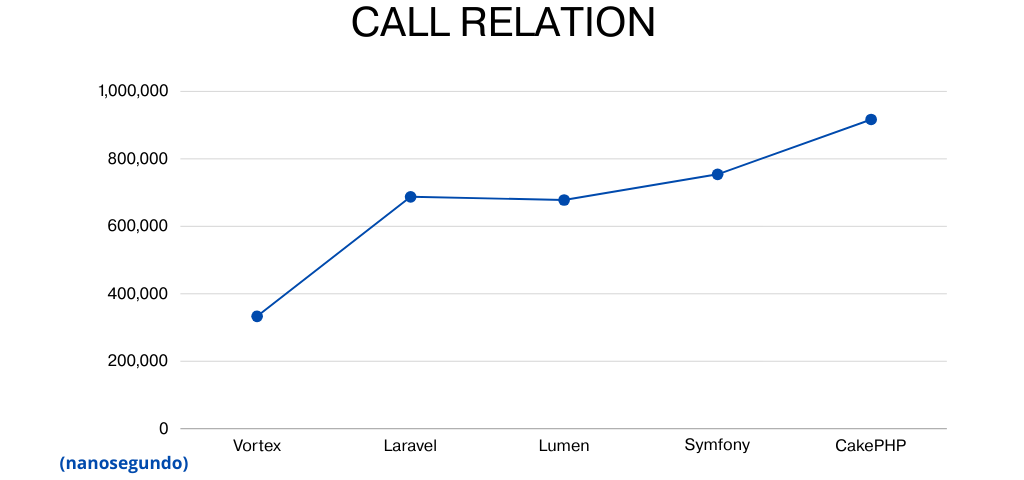
\includegraphics[width=0.9\linewidth]{figures/call_relations.png}
    \caption{Gráfico comparativo performance ORM dos \textit{frameworks} em relacionamentos}
    \label{fig:call_relations}
\end{figure}

\begin{table}[H] \footnotesize
\fontsize{9pt}{9pt}\selectfont
\centering
\vspace{1cm}
\begin{tabular}{|c|c|c|c|}
\hline
Framework & Tempo de Execução(ns)\\
\hline 
Vortex  & 333283 ns \\
Laravel & 687478 ns \\
Lumen   & 678044 ns \\
Symfony & 754170 ns \\
CakePHP & 916754 ns \\
\hline
\end{tabular}
\caption{Tempo de execução consultas de relacionamentos entre os \textit{frameworks}}
\label{call_relations_table}
\end{table}

\begin{figure}[H]
    \centering
    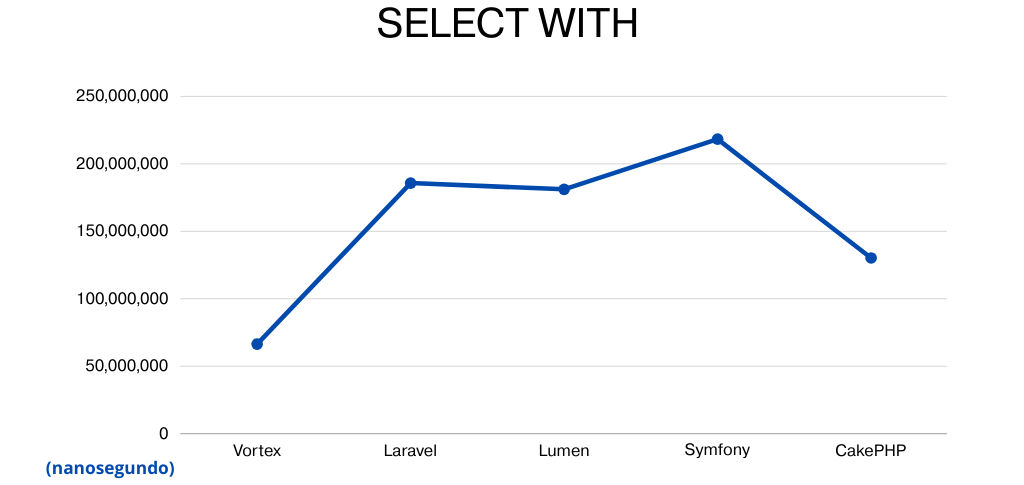
\includegraphics[width=0.9\linewidth]{figures/select_with.png}
    \caption{Gráfico comparativo performance ORM dos \textit{frameworks} em relacionamentos carregados na entidade primaria}
    \label{fig:select_with}
\end{figure}

\begin{table}[H] \footnotesize
\fontsize{9pt}{9pt}\selectfont
\centering
\vspace{1cm}
\begin{tabular}{|c|c|c|c|}
\hline
Framework & Tempo de Execução(ns)\\
\hline 
Vortex  & 66426900 ns \\
Laravel & 185758000 ns \\
Lumen   & 181123000 ns \\
Symfony & 218312000 ns \\
CakePHP & 130254000 ns \\
\hline
\end{tabular}
\caption{Tempo de execução entre os \textit{frameworks} em consultas de entidades carregando relacionamentos}
\label{select_with_table}
\end{table}

Com base nos dados expostos nas tabelas, é possível inferir que, em ambas as consultas, observou-se uma superioridade do Vortex em comparação aos demais \textit{frameworks}. No contexto da Tabela \ref{call_relations_table}, na consulta denominada \textit{CALL RELATION}, registrou-se o menor tempo de execução após a utilização do Vortex, sendo o Lumen aquele que apresentou aproximadamente $\approx$ 2,034 vezes o tempo de execução do Vortex. Por outro lado, o CakePHP evidenciou o desempenho menos favorável, apresentando um tempo de execução aproximadamente $\approx$ 2,750 vezes superior ao do Vortex. Já em consultas \textit{SELECT WITH} também se observa a vantagem do Vortex em relação ados demais \textit{frameworks}, sendo novamente o pior comparado foi o Symfony com 218312000 ns e aproximadamente $\approx$ 3,286 vezes mais lento que o Vortex. Já o melhor comparado ao Vortex foi o Lumen com 181123000 ns e $\approx$ 2,726 vezes o tempo de execução do Vortex.

Os resultados dos testes práticos são ilustrados nas figuras: \ref{fig:vortex_vs_cakephp}, \ref{fig:vortex_vs_lumen}, \ref{fig:vortex_vs_symfony}, \ref{fig:vortex_vs_laravel}, \ref{fig:call_relations} e \ref{fig:select_with}, evidenciando a superioridade de desempenho do Vortex em comparação com outros \textit{frameworks}. Com o mesmo propósito de avaliação dos parâmetros de performance, a análise se concentra no tempo de execução de rotinas específicas em cada \textit{framework}, focalizando a comparação entre Vortex e Laravel. Os dados apresentados nas tabelas \ref{vortex_vs_laravel} são confrontados em termos de nanossegundos, sendo que a última coluna à direita representa a razão relativa ao tempo de execução do Laravel em relação ao Vortex. Dessa maneira, é possível observar quantas vezes as rotinas do Laravel demandaram mais tempo do que as correspondentes no Vortex. Já as consultas de relacionamentos mostraram vantagem para o Vortex em relação ao Laravel na ordem de $\approx$ 2,062 para o cenário de \textit{CALL RELATION} e para \textit{SELECT WITH} $\approx$ 2,796.